\documentclass{beamer}
\usepackage[english,russian]{babel}
\usepackage[utf8]{inputenc}
\usepackage{amsmath}
\usepackage{hyperref}
\usetheme{Warsaw}
\usepackage{listings}
\usepackage{xcolor}
\usepackage{tikz}
\usetikzlibrary{graphs}
\usepackage{algpseudocode}

\lstset{
    frame=tb,
    tabsize=4,
    showstringspaces=false,
    numbers=left,
    commentstyle=\color{green},
    keywordstyle=\color{blue},
    stringstyle=\color{red},
    emph={baz},
    emphstyle=\textbf
}
\begin{document}

\title{Задачи разрешимости логических формул и приложения\newline Лекция 11. Символическое исполнение}
\author{Роман Холин}
\institute{Московский государственный университет}
\date{Москва, 2022}

\begin{frame}
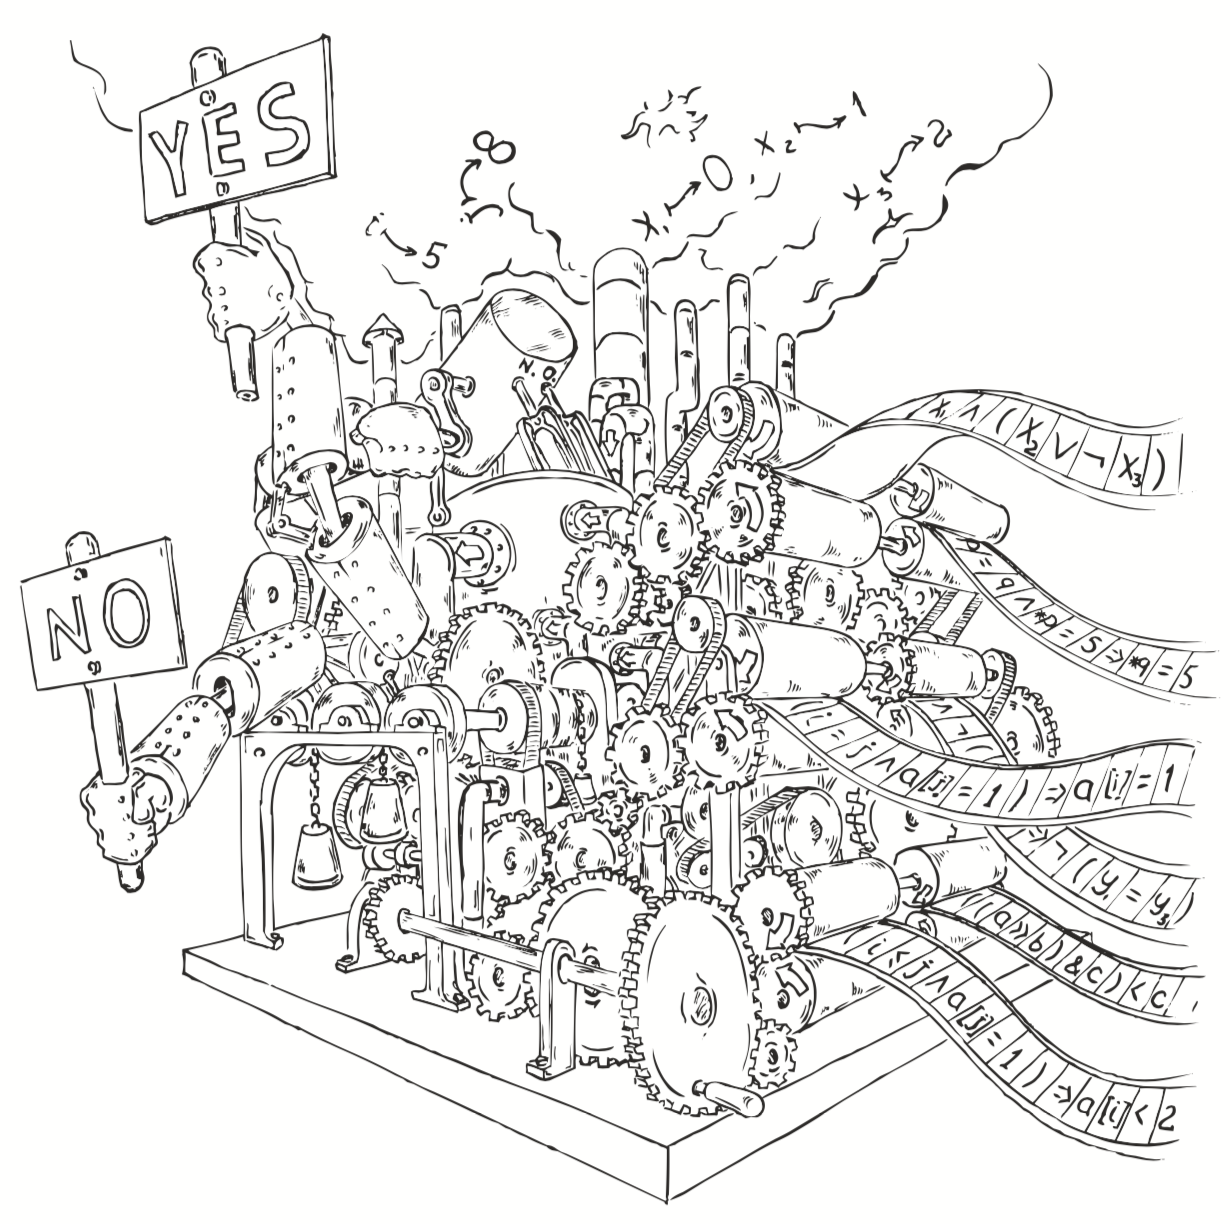
\includegraphics[scale=0.5]{../decision-procedure.png}
\end{frame}

\frame{\titlepage}

\begin{frame}{Мотивация}
\begin{itemize}
\item Хочется автоматизировать генерацию тестовых примеров
\end{itemize}
\end{frame}

\begin{frame}{Мотивация}
\begin{itemize}
\item Хочется автоматизировать генерацию тестовых примеров
\item Хочется, чтобы тесты посещали все строчки кода (LOC метрика)
\end{itemize}
\end{frame}

\begin{frame}{Мотивация}
\begin{itemize}
\item Хочется автоматизировать генерацию тестовых примеров
\item Хочется, чтобы тесты посещали все строчки кода (LOC метрика)
\item Хочется, чтобы тесты посещали все пути обхода программы
\end{itemize}
\end{frame}

\begin{frame}{Что можно делать}
\begin{itemize}
\item Dynamic analysis
\item Program correctness
\item Test generations
\item Taint analysis
\end{itemize}
\end{frame}

\begin{frame}[fragile]{Конкретное исполнение (Concrete execution)}
\begin{minipage}{0.49\textwidth}
\begin{lstlisting}[language=C++]
void foo(int x, int y) {
    int t = 0;
    if (x > y) {
        t = x;
    } else {
        t = y;
    }
    if (t < x) {
        assert false;
    }
}
\end{lstlisting}
\end{minipage}
\hfill
\begin{minipage}{0.49\textwidth}
\begin{center}
\begin{tabular}{ | l | l | l | }
\hline
$X$ & $Y$ & $T$ \\
\hline
4 & 4 & 0 \\
\hline
\end{tabular}
\end{center}
\end{minipage}
\end{frame}

\begin{frame}[fragile]{Конкретное исполнение (Concrete execution)}
\begin{minipage}{0.49\textwidth}
\begin{lstlisting}[language=C++]
void foo(int x, int y) {
    int t = 0;
    //if (x > y) {
    //    t = x;
    //} else {
        t = y;
    //}
    if (t < x) {
        assert false;
    }
}
\end{lstlisting}
\end{minipage}
\hfill
\begin{minipage}{0.49\textwidth}
\begin{center}
\begin{tabular}{ | l | l | l | }
\hline
$X$ & $Y$ & $T$ \\
\hline
4 & 4 & 4 \\
\hline
\end{tabular}
\end{center}
\end{minipage}
\end{frame}

\begin{frame}[fragile]{Конкретное исполнение (Concrete execution)}
\begin{minipage}{0.49\textwidth}
\begin{lstlisting}[language=C++]
void foo(int x, int y) {
    int t = 0;
    if (x > y) {
        t = x;
    } else {
        t = y;
    }
    if (t < x) {
        assert false;
    }
}
\end{lstlisting}
\end{minipage}
\hfill
\begin{minipage}{0.49\textwidth}
\begin{center}
\begin{tabular}{ | l | l | l | }
\hline
$X$ & $Y$ & $T$ \\
\hline
2 & 1 & 0 \\
\hline
\end{tabular}
\end{center}
\end{minipage}
\end{frame}

\begin{frame}[fragile]{Конкретное исполнение (Concrete execution)}
\begin{minipage}{0.49\textwidth}
\begin{lstlisting}[language=C++]
void foo(int x, int y) {
    int t = 0;
    //if (x > y) {
        t = x;
    //} else {
    //    t = y;
    //}
    if (t < x) {
        assert false;
    }
}
\end{lstlisting}
\end{minipage}
\hfill
\begin{minipage}{0.49\textwidth}
\begin{center}
\begin{tabular}{ | l | l | l | }
\hline
$X$ & $Y$ & $T$ \\
\hline
2 & 1 & 2 \\
\hline
\end{tabular}
\end{center}
\end{minipage}
\end{frame}

\begin{frame}{Пути исполнения программы}
\begin{minipage}{0.49\textwidth}
\begin{itemize}
\item Программа может быть представленна в виде бинарного дерева - т.н. Вычислительного дерева
\item Каждая вершина - выполнение условного оператора
\item Каждое ребро - выполнение последователнисти команд, которые не являются условным оператором
\item Кадый путь от корня - делит множество входных данных на классы эквивалентности
\end{itemize}
\end{minipage}
\begin{minipage}{0.49\textwidth}
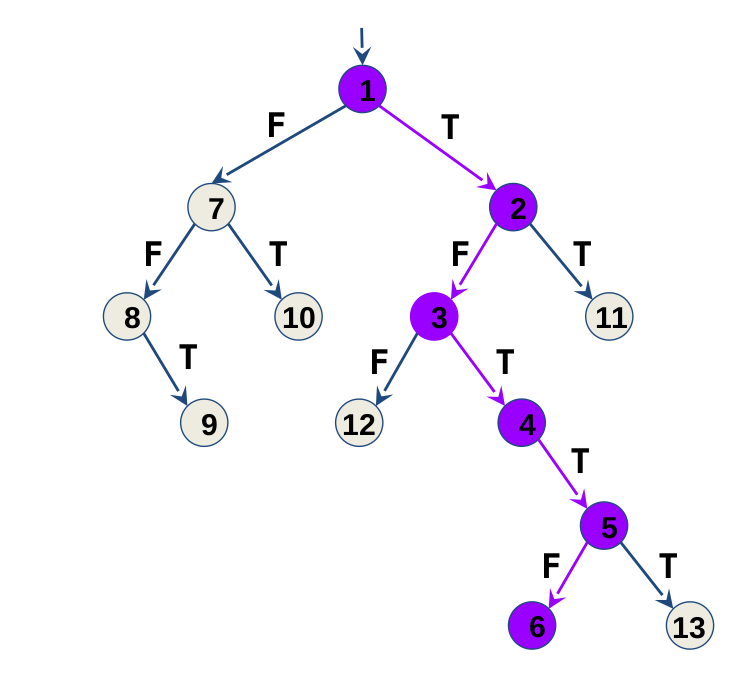
\includegraphics[scale=0.2]{tree.png}
\end{minipage}
\end{frame}

\begin{frame}[fragile]{Пример дерева}
\begin{minipage}{0.49\textwidth}
\begin{lstlisting}[language=C++]
void test(int x, int y) {
   if (2*y == x) {
      if (x <= y+10) {
         printf("OK");
      } else {
         printf("not OK");
         assert false;
      }
   } else {
      print("OK");
   }
}
\end{lstlisting}
\end{minipage}
\end{frame}

\begin{frame}[fragile]{Существующие подходы}
\begin{minipage}{0.49\textwidth}
\begin{lstlisting}[language=C++]
 void test(int x) {
     if (x == 94389) {
         assert false;
     }
 }
\end{lstlisting}
\end{minipage}
\begin{minipage}{0.49\textwidth}
\begin{itemize}
\item Рандомизированное тестирование
\item Проблема: вероятность ошибка очень мала
\end{itemize}
\end{minipage}
\end{frame}

\begin{frame}[fragile]{Символическое исполнение (Symbolic execution)}
\begin{minipage}{0.49\textwidth}
\begin{lstlisting}[language=C++]
void foo(int x, int y) {
    int t = 0;
    if (x > y) {
        t = x;
    } else {
        t = y;
    }
    if (t < x) {
        assert false;
    }
}
\end{lstlisting}
\end{minipage}
\hfill
\begin{minipage}{0.49\textwidth}
\begin{center}
\begin{tabular}{ | l | l | l | }
\hline
$X$ & $Y$ & $T$ \\
\hline
$x$ & $y$ & 0 \\
\hline
\end{tabular}
\end{center}
\end{minipage}
\end{frame}

\begin{frame}[fragile]{Символическое исполнение (Symbolic execution)}
\begin{minipage}{0.49\textwidth}
\begin{lstlisting}[language=C++]
void foo(int x, int y) {
    int t = 0;
    if (x > y) {
        t = x;
    } else {
        t = y;
    }
    if (t < x) {
        assert false;
    }
}
\end{lstlisting}
\end{minipage}
\hfill
\begin{minipage}{0.49\textwidth}
\begin{center}
\begin{tabular}{ | l | l | l | }
\hline
$X$ & $Y$ & $T$ \\
\hline
$x$ & $y$ & $t_0$ \\
\hline
\end{tabular}
\begin{equation*}
t_0 =
    \begin{cases}
    $x$ &\text{$x > y$}\\
    $y$ &\text{$x \le y$}
    \end{cases}
\end{equation*}
\end{center}
\end{minipage}
\end{frame}

\begin{frame}[fragile]{Символическое исполнение (Symbolic execution)}
\begin{minipage}{0.49\textwidth}
\begin{lstlisting}[language=C++]
void foo(int x, int y) {
    int t = 0;
    if (x > y) {
        t = x;
    } else {
        t = y;
    }
    if (t < x) {
        assert false;
    }
}
\end{lstlisting}
\end{minipage}
\hfill
\begin{minipage}{0.49\textwidth}
\begin{center}
\begin{tabular}{ | l | l | l | }
\hline
$X$ & $Y$ & $T$ \\
\hline
$x$ & $y$ & $t_0$ \\
\hline
\end{tabular}
\begin{equation*}
t_0 =
    \begin{cases}
    $x$ &\text{$x > y$}\\
    $y$ &\text{$x \le y$}
    \end{cases}
\end{equation*}
$t_0 < x?$
\end{center}
\end{minipage}
\end{frame}

\begin{frame}[fragile]{Символическое исполнение (Symbolic execution)}
\begin{minipage}{0.49\textwidth}
\begin{lstlisting}[language=C++]
void foo(int x, int y) {
    int t = 0;
    if (x > y) {
        t = x;
    } else {
        t = y;
    }
    if (t < x) {
        assert false;
    }
}
\end{lstlisting}
\end{minipage}
\hfill
\begin{minipage}{0.49\textwidth}
\begin{center}
\begin{tabular}{ | l | l | l | }
\hline
$X$ & $Y$ & $T$ \\
\hline
$x$ & $y$ & $t_0$ \\
\hline
\end{tabular}
\begin{equation*}
t_0 =
    \begin{cases}
    $x$ &\text{$x > y$}\\
    $y$ &\text{$x \le y$}
    \end{cases}
\end{equation*}
$\left\{
\begin{array}{l}
x > y \implies t_0 = x \implies t_0 \ge x \\
x \le y \implies t_0 = y \implies t_0 \ge x \\
\end{array}
\right.$
\end{center}
\end{minipage}
\end{frame}

\begin{frame}[fragile]{Символическое исполнение (Symbolic execution)}
\begin{minipage}{0.49\textwidth}
\begin{lstlisting}[language=C++]
void foo(int x, int y) {
    int t = 0;
    if (x > y) {
        t = x - 1;
    } else {
        t = y;
    }
    if (t < x) {
        assert false;
    }
}
\end{lstlisting}
\end{minipage}
\hfill
\begin{minipage}{0.49\textwidth}
\begin{center}
\begin{tabular}{ | l | l | l | }
\hline
$X$ & $Y$ & $T$ \\
\hline
$x$ & $y$ & $t_0$ \\
\hline
\end{tabular}
\end{center}
\end{minipage}
\end{frame}

\begin{frame}[fragile]{Символическое исполнение (Symbolic execution)}
\begin{minipage}{0.49\textwidth}
\begin{lstlisting}[language=C++]
void foo(int x, int y) {
    int t = 0;
    if (x > y) {
        t = x - 1;
    } else {
        t = y;
    }
    if (t < x) {
        assert false;
    }
}
\end{lstlisting}
\end{minipage}
\hfill
\begin{minipage}{0.49\textwidth}
\begin{center}
\begin{tabular}{ | l | l | l | }
\hline
$X$ & $Y$ & $T$ \\
\hline
$x$ & $y$ & $t_0$ \\
\hline
\end{tabular}
\begin{equation*}
t_0 =
    \begin{cases}
    $x - 1$ &\text{$x > y$}\\
    $y$ &\text{$x \le y$}
    \end{cases}
\end{equation*}
\end{center}
\end{minipage}
\end{frame}

\begin{frame}[fragile]{Символическое исполнение (Symbolic execution)}
\begin{minipage}{0.49\textwidth}
\begin{lstlisting}[language=C++]
void foo(int x, int y) {
    int t = 0;
    //if (x > y) {
        t = x - 1;
    //} else {
    //    t = y;
    //}
    //if (t < x) {
        assert false;
    //}
}
\end{lstlisting}
\end{minipage}
\hfill
\begin{minipage}{0.49\textwidth}
\begin{center}
\begin{tabular}{ | l | l | l | }
\hline
$X$ & $Y$ & $T$ \\
\hline
$x$ & $y$ & $t_0$ \\
\hline
\end{tabular}
\begin{equation*}
t_0 =
    \begin{cases}
    $x - 1$ &\text{$x > y$}\\
    $y$ &\text{$x \le y$}
    \end{cases}
\end{equation*}
$\left\{
\begin{array}{l}
x > y \implies t_0 = x - 1 \implies t_0 < x \\
x \le y \implies t_0 = y \implies t_0 \ge x \\
\end{array}
\right.$
$x > y$ - solution
\end{center}
\end{minipage}
\end{frame}

\begin{frame}[fragile]{Символическое исполнение (Symbolic execution)}
\begin{minipage}{0.49\textwidth}
\begin{lstlisting}[language=C++]
void testme(int x) {
   if (pow(2,x) % c == 17) {
      printf("not OK");
      assert false;
   } else
      printf("OK");
}
\end{lstlisting}
\end{minipage}
\end{frame}


\begin{frame}[fragile]{Concolic execution}
Concolic execution (или dynamic symbolic execution):
\begin{itemize}
\item Начнем с рандомных входных данных
\item Поддерживаем конкретный и символьные переменные
\end{itemize}
\end{frame}

\begin{frame}[fragile]{Concolic execution}
\begin{minipage}{0.49\textwidth}
\begin{lstlisting}[language=C++,escapechar=@]
void foo(int x, int y) {
    int t = 0;
    if (x > y) {
        t = x;
    } else {
        t = y;
    }
    if (t < x) {
        assert false;
    }
}
\end{lstlisting}
\end{minipage}
\hfill
\begin{minipage}{0.49\textwidth}
\begin{center}
\begin{tabular}{ | l | l | l | }
\hline
$X$ & $Y$ & $T$ \\
\hline
$x$ & $y$ & $t_0$ \\
\hline
\end{tabular}
\begin{equation*}
t_0 =
    \begin{cases}
    $x$ &\text{$x > y$}\\
    $y$ &\text{$x \le y$}
    \end{cases}
\end{equation*}
\end{center}
\end{minipage}
\end{frame}

\begin{frame}[fragile]{Concolic execution}
\begin{minipage}{0.49\textwidth}
\begin{lstlisting}[language=C++,escapechar=@]
void foo(int x, int y) {
    @\textbf{int t = 0;}@
    if (x > y) {
        t = x;
    } else {
        t = y;
    }
    if (t < x) {
        assert false;
    }
}
\end{lstlisting}
\end{minipage}
\hfill
\begin{minipage}{0.49\textwidth}
\begin{center}
\begin{tabular}{ | l | l | l | }
\hline
$X$ & $Y$ & $T$ \\
\hline
$(0, x)$ & $(0, y)$ & $(0, 0)$ \\
\hline
\end{tabular}
\end{center}
\end{minipage}
\end{frame}

\begin{frame}[fragile]{Concolic execution}
\begin{minipage}{0.49\textwidth}
\begin{lstlisting}[language=C++,escapechar=@]
void foo(int x, int y) {
    @\textbf{int t = 0;}@
    @\textbf{if (x > y) \{}@
        t = x;
    } else {
        t = y;
    }
    if (t < x) {
        assert false;
    }
}
\end{lstlisting}
\end{minipage}
\hfill
\begin{minipage}{0.49\textwidth}
\begin{center}
\begin{tabular}{ | l | l | l | }
\hline
$X$ & $Y$ & $T$ \\
\hline
$(0, x)$ & $(0, y)$ & $(0, 0)$ \\
\hline
\end{tabular}
\end{center}
\end{minipage}
\end{frame}

\begin{frame}[fragile]{Concolic execution}
\begin{minipage}{0.49\textwidth}
\begin{lstlisting}[language=C++,escapechar=@]
void foo(int x, int y) {
    @\textbf{int t = 0;}@
    @\textbf{if (x > y) \{}@
        t = x;
    } else {
        t = y;
    }
    if (t < x) {
        assert false;
    }
}
\end{lstlisting}
\end{minipage}
\hfill
\begin{minipage}{0.49\textwidth}
\begin{center}
\begin{tabular}{ | l | l | l | }
\hline
$X$ & $Y$ & $T$ \\
\hline
$(0, x)$ & $(0, y)$ & $(0, 0)$ \\
\hline
\end{tabular}
$\left\{
\begin{array}{l}
F1 = not (x > y)
\end{array}
\right.$
\end{center}
\end{minipage}
\end{frame}

\begin{frame}[fragile]{Concolic execution}
\begin{minipage}{0.49\textwidth}
\begin{lstlisting}[language=C++,escapechar=@]
void foo(int x, int y) {
    @\textbf{int t = 0;}@
    @\textbf{if (x > y) \{}@
        t = x;
    } else {
        t = y;
    }
    if (t < x) {
        assert false;
    }
}
\end{lstlisting}
\end{minipage}
\hfill
\begin{minipage}{0.49\textwidth}
\begin{center}
\begin{tabular}{ | l | l | l | }
\hline
$X$ & $Y$ & $T$ \\
\hline
$(0, x)$ & $(0, y)$ & $(0, 0)$ \\
\hline
\end{tabular}
$\left\{
\begin{array}{l}
F1 = not (x > y)
\end{array}
\right.$
$SMT\_Solver($not $F1) \to (x = 1, y = 0)$
\end{center}
\end{minipage}
\end{frame}

\begin{frame}[fragile]{Concolic execution}
\begin{minipage}{0.49\textwidth}
\begin{lstlisting}[language=C++,escapechar=@]
void foo(int x, int y) {
    @\textbf{int t = 0;}@
    @\textbf{if (x > y) \{}@
        t = x;
    } else {
        t = y;
    }
    if (t < x) {
        assert false;
    }
}
\end{lstlisting}
\end{minipage}
\hfill
\begin{minipage}{0.49\textwidth}
\begin{center}
\begin{tabular}{ | l | l | l | }
\hline
$X$ & $Y$ & $T$ \\
\hline
$(0, x)$ & $(0, y)$ & $(0, 0)$ \\
\hline
\end{tabular}
$\left\{
\begin{array}{l}
F1 = not (x > y)
\end{array}
\right.$
$SMT\_Solver($not $F1) \to (x = 1, y = 0)$
$queue = \{(x = 1, y = 0)\}$
\end{center}
\end{minipage}
\end{frame}

\begin{frame}[fragile]{Concolic execution}
\begin{minipage}{0.49\textwidth}
\begin{lstlisting}[language=C++,escapechar=@]
void foo(int x, int y) {
    @\textbf{int t = 0;}@
    @\textbf{if (x > y) \{}@
        t = x;
    @\textbf{\} else \{}@
        t = y;
    }
    if (t < x) {
        assert false;
    }
}
\end{lstlisting}
\end{minipage}
\hfill
\begin{minipage}{0.49\textwidth}
\begin{center}
\begin{tabular}{ | l | l | l | }
\hline
$X$ & $Y$ & $T$ \\
\hline
$(0, x)$ & $(0, y)$ & $(0, 0)$ \\
\hline
\end{tabular}
$\left\{
\begin{array}{l}
F1 = not (x > y)
\end{array}
\right.$
$queue = \{(x = 1, y = 0)\}$
\end{center}
\end{minipage}
\end{frame}

\begin{frame}[fragile]{Concolic execution}
\begin{minipage}{0.49\textwidth}
\begin{lstlisting}[language=C++,escapechar=@]
void foo(int x, int y) {
    @\textbf{int t = 0;}@
    @\textbf{if (x > y) \{}@
        t = x;
    @\textbf{\} else \{}@
        @\textbf{t = y;}@
    }
    if (t < x) {
        assert false;
    }
}
\end{lstlisting}
\end{minipage}
\hfill
\begin{minipage}{0.49\textwidth}
\begin{center}
\begin{tabular}{ | l | l | l | }
\hline
$X$ & $Y$ & $T$ \\
\hline
$(0, x)$ & $(0, y)$ & $(0, y)$ \\
\hline
\end{tabular}
$\left\{
\begin{array}{l}
F1 = not (x > y)
\end{array}
\right.$
$queue = \{(x = 1, y = 0)\}$
\end{center}
\end{minipage}
\end{frame}

\begin{frame}[fragile]{Concolic execution}
\begin{minipage}{0.49\textwidth}
\begin{lstlisting}[language=C++,escapechar=@]
void foo(int x, int y) {
    @\textbf{int t = 0;}@
    @\textbf{if (x > y) \{}@
        t = x;
    @\textbf{\} else \{}@
        @\textbf{t = y;}@
    @\textbf{\}}@
    if (t < x) {
        assert false;
    }
}
\end{lstlisting}
\end{minipage}
\hfill
\begin{minipage}{0.49\textwidth}
\begin{center}
\begin{tabular}{ | l | l | l | }
\hline
$X$ & $Y$ & $T$ \\
\hline
$(0, x)$ & $(0, y)$ & $(0, y)$ \\
\hline
\end{tabular}
$\left\{
\begin{array}{l}
F1 = not (x > y)
\end{array}
\right.$
$queue = \{(x = 1, y = 0)\}$
\end{center}
\end{minipage}
\end{frame}

\begin{frame}[fragile]{Concolic execution}
\begin{minipage}{0.49\textwidth}
\begin{lstlisting}[language=C++,escapechar=@]
void foo(int x, int y) {
    @\textbf{int t = 0;}@
    @\textbf{if (x > y) \{}@
        t = x;
    @\textbf{\} else \{}@
        @\textbf{t = y;}@
    @\textbf{\}}@
    @\textbf{if (t < x) \{}@
        assert false;
    }
}
\end{lstlisting}
\end{minipage}
\hfill
\begin{minipage}{0.49\textwidth}
\begin{center}
\begin{tabular}{ | l | l | l | }
\hline
$X$ & $Y$ & $T$ \\
\hline
$(0, x)$ & $(0, y)$ & $(0, y)$ \\
\hline
\end{tabular}
$\left\{
\begin{array}{l}
F1 = not (x > y)
\end{array}
\right.$
$queue = \{(x = 1, y = 0)\}$
\end{center}
\end{minipage}
\end{frame}

\begin{frame}[fragile]{Concolic execution}
\begin{minipage}{0.49\textwidth}
\begin{lstlisting}[language=C++,escapechar=@]
void foo(int x, int y) {
    @\textbf{int t = 0;}@
    @\textbf{if (x > y) \{}@
        t = x;
    @\textbf{\} else \{}@
        @\textbf{t = y;}@
    @\textbf{\}}@
    @\textbf{if (t < x) \{}@
        assert false;
    }
}
\end{lstlisting}
\end{minipage}
\hfill
\begin{minipage}{0.49\textwidth}
\begin{center}
\begin{tabular}{ | l | l | l | }
\hline
$X$ & $Y$ & $T$ \\
\hline
$(0, x)$ & $(0, y)$ & $(0, y)$ \\
\hline
\end{tabular}
$\left\{
\begin{array}{l}
F1 = not (x > y) \\
F2 = not (y < x)
\end{array}
\right.$
$queue = \{(x = 1, y = 0)\}$
\end{center}
\end{minipage}
\end{frame}

\begin{frame}[fragile]{Concolic execution}
\begin{minipage}{0.49\textwidth}
\begin{lstlisting}[language=C++,escapechar=@]
void foo(int x, int y) {
    @\textbf{int t = 0;}@
    @\textbf{if (x > y) \{}@
        t = x;
    @\textbf{\} else \{}@
        @\textbf{t = y;}@
    @\textbf{\}}@
    @\textbf{if (t < x) \{}@
        assert false;
    }
}
\end{lstlisting}
\end{minipage}
\hfill
\begin{minipage}{0.49\textwidth}
\begin{center}
\begin{tabular}{ | l | l | l | }
\hline
$X$ & $Y$ & $T$ \\
\hline
$(0, x)$ & $(0, y)$ & $(0, y)$ \\
\hline
\end{tabular}
$\left\{
\begin{array}{l}
F1 = not (x > y) \\
F2 = not (y < x)
\end{array}
\right.$
$SMT\_Solver(F1$ and not $F2) \to UNSAT$
$queue = \{(x = 1, y = 0)\}$
\end{center}
\end{minipage}
\end{frame}

\begin{frame}[fragile]{Concolic execution}
\begin{minipage}{0.49\textwidth}
\begin{lstlisting}[language=C++,escapechar=@]
void foo(int x, int y) {
    @\textbf{int t = 0;}@
    @\textbf{if (x > y) \{}@
        t = x;
    @\textbf{\} else \{}@
        @\textbf{t = y;}@
    @\textbf{\}}@
    @\textbf{if (t < x) \{}@
        assert false;
    @\textbf{\}}@
}
\end{lstlisting}
\end{minipage}
\hfill
\begin{minipage}{0.49\textwidth}
\begin{center}
\begin{tabular}{ | l | l | l | }
\hline
$X$ & $Y$ & $T$ \\
\hline
$(0, x)$ & $(0, y)$ & $(0, y)$ \\
\hline
\end{tabular}
$\left\{
\begin{array}{l}
F1 = not (x > y) \\
F2 = not (y < x)
\end{array}
\right.$
$queue = \{(x = 1, y = 0)\}$
\end{center}
\end{minipage}
\end{frame}

\begin{frame}[fragile]{Concolic execution}
\begin{minipage}{0.49\textwidth}
\begin{lstlisting}[language=C++,escapechar=@]
void foo(int x, int y) {
    int t = 0;
    if (x > y) {
        t = x;
    } else {
        t = y;
    }
    if (t < x) {
        assert false;
    }
}
\end{lstlisting}
\end{minipage}
\hfill
\begin{minipage}{0.49\textwidth}
\begin{center}
\begin{tabular}{ | l | l | l | }
\hline
$X$ & $Y$ & $T$ \\
\hline
$(1, x)$ & $(0, y)$ & $(0, 0)$ \\
\hline
\end{tabular}
$queue = \{\}$
\end{center}
\end{minipage}
\end{frame}

\begin{frame}{Пример}
Какие ограничения могут повстречатся при consolic execution?
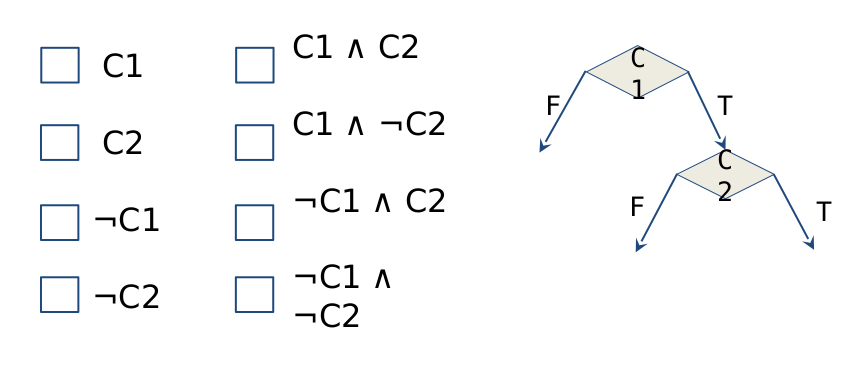
\includegraphics[scale=0.35]{quiz.png}
\end{frame}

\begin{frame}[fragile]{Пример}
\begin{minipage}{0.49\textwidth}
\begin{lstlisting}[language=C++]
int test(int x) {
   int[] A = { 5, 7, 9 };
   int i = 0;
   while (i < 3) {
      if (A[i] == x) {
          break;
      }
      i++;
   }
   return i;
}
\end{lstlisting}
\end{minipage}
\begin{minipage}{0.49\textwidth}
Какие ограничения появлялись и были разрешены солвером?
\end{minipage}
\end{frame}

\begin{frame}[fragile]{Пример}
\begin{minipage}{0.40\textwidth}
\begin{lstlisting}[language=C++]
int foo(int v) {
   return secure_hash(v);
}

void test(int x, int y) {
   if (x != y)
      if (foo(x) == foo(y))
         assert;
}
\end{lstlisting}
\end{minipage}
\hfill
\begin{minipage}{0.40\textwidth}
Можно символические переменные заменить на конкретные
\end{minipage}
\end{frame}

\begin{frame}{Преимущества и недостатки Consolic Execution}
\begin{itemize}
\item Может никогда не остановиться
\item Метод полный - если мы достигаем ошибки, то программа достигает её на некоторых данных
\item Не надежный - если анализ останавливается и не нашёл ошибок, то это не значит, что их нет
\end{itemize}
\end{frame}

\begin{frame}[fragile]{Реализация}
\begin{lstlisting}[language=python,escapechar=@]
a = b + c
\end{lstlisting}
\end{frame}

\begin{frame}[fragile]{Реализация}
\begin{lstlisting}[language=python,escapechar=@]
class concolic_int(int):
def __new__(cls, val, sym):
    self =
     super(concolic_int, cls).__new__(cls, val)
    self.__val = val
    self.__sym = sym
    return self
def __add__(self, other):
    if isinstance(other, concolic_int):
        value = self.__val + other.__val
        symbolic = self.__sym + "+" + other.__sym
    else:
        value = self.__val + other
        symbolic = self.__sym + "+" + str(other)
    return concolic_int(value, symbolic)
\end{lstlisting}
\end{frame}

\begin{frame}[fragile]{Реализация}
Как int заменить на concolic\_int?
\end{frame}

\begin{frame}[fragile]{Реализация}
\begin{lstlisting}[language=python,escapechar=@]
a = b + c
\end{lstlisting}
\end{frame}

\begin{frame}[fragile]{Реализация}
\begin{lstlisting}[language=python,escapechar=@]
a = plus(b, c)
\end{lstlisting}
\end{frame}

\begin{frame}[fragile]{Реализация}
\begin{lstlisting}[language=python,escapechar=@]
function plus(x, y) {
    if (x isinstanceof Concolic) {
        if (y isinstanceof Concolic) {
            return new Concolic(
                x._val + y._val,
                x._sym + "+" + y._sym
            );
        } else {
            return new Concolic(
                x._val + y,
                x._sym + "+" + y.toString()
            );
        }
    } else {
        ....
    }
}
\end{lstlisting}
\end{frame}

\begin{frame}[fragile]{Реализация}
Как кодировать пути?
\end{frame}

\begin{frame}{Examples}
\begin{itemize}
\item KLEE: LLVM (C family of languages)
\item PEX: .NET Framework
\item CUTE: C
\item jCUTE: Java
\item Jalangi: Javascript
\item Jalangi2 + ExpoSE: Javascript
\item SAGE and S2E: binaries (x86, ARM, ...)
\end{itemize}
\end{frame}

\begin{frame}{Links}
\begin{itemize}
\item https://www.youtube.com/watch?v=yRVZPvHYHzw - MIT lecture
\item Symbolic Execution and Program Testing. James C. King
\item SAGE: Whitebox Fuzzing for Security Testing. Patrice Godefroid, Michael Y. Levin, and David A. Molnar
\item Jalangi: A Selective Record-Replay and Dynamic Analysis Framework for JavaScript. Koushik Sen, Swaroop Kalasapur, Tasneem Brutch, Simon Gibbs
\item Sound Regular Expression Semantics for Dynamic Symbolic Execution of JavaScript. Blake Loring, Duncan Mitchell, Johannes Kinder
\end{itemize}
\end{frame}

\begin{frame}
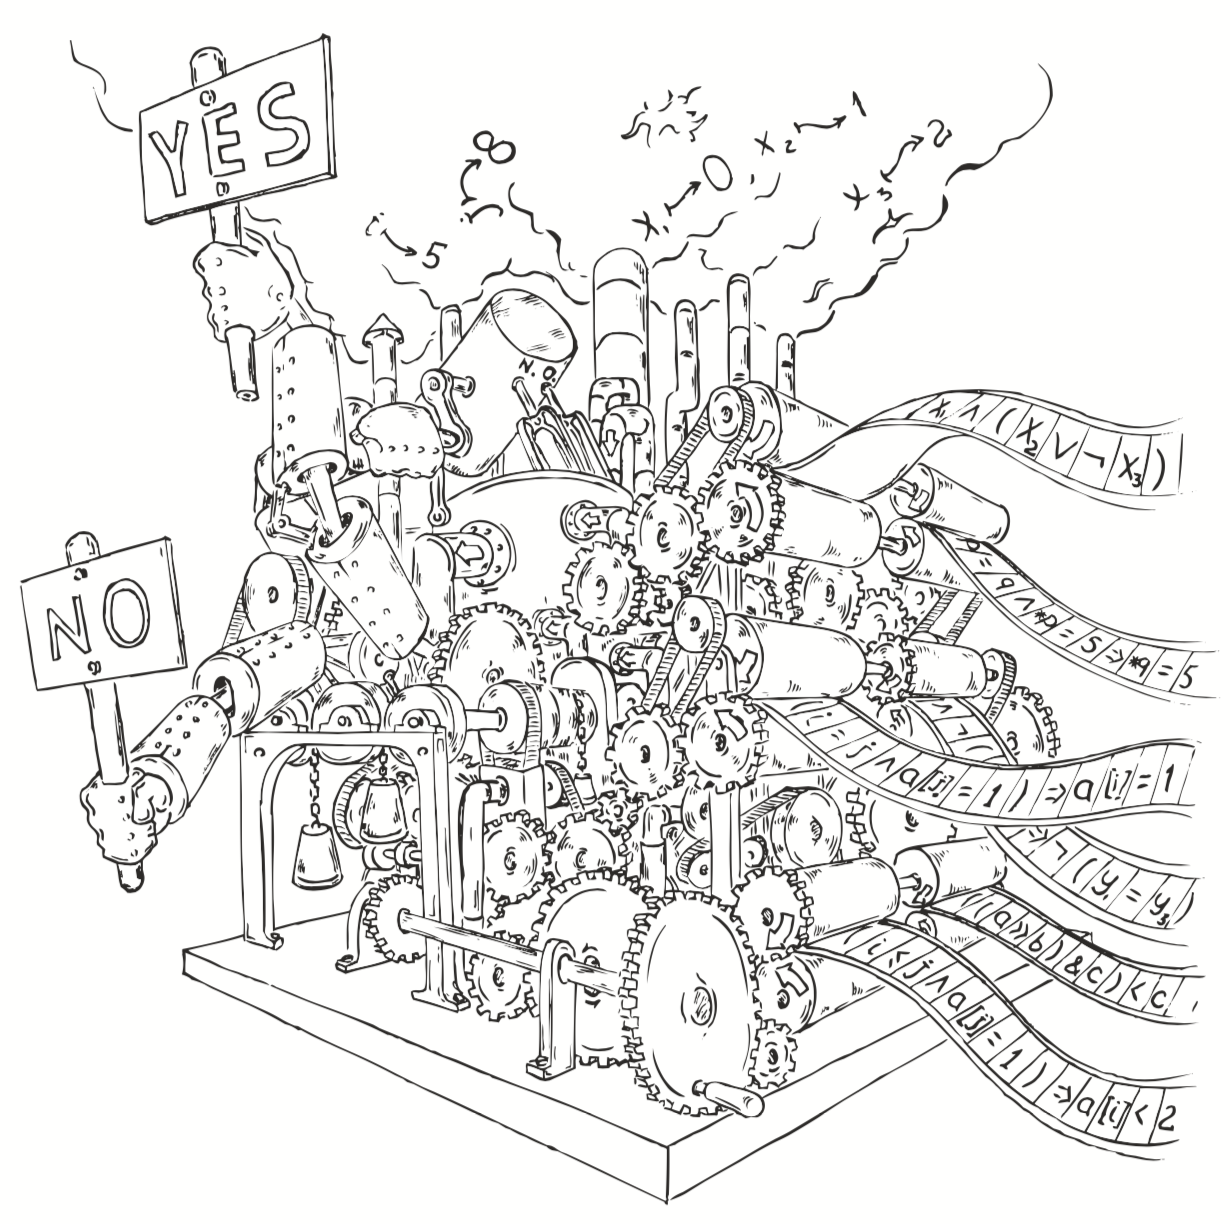
\includegraphics[scale=0.5]{../decision-procedure.png}
\end{frame}

\end{document}
